\section{Mediciones}

\subsection{Construcción de las entradas}

Para generar los archivos de entrada hicimos un script en lenguaje Python.

El primer bloque de código genera un archivo llamado ``medicionesConSpanVariable.in''. Se fijan primero las constantes \emph{h}, \emph{carga}, \emph{C} y \emph{fMax}
(Las dos últimas no serán utilizadas, se agregan por consistencia, la carga se usará para todas las juntas por igual y será fija, al igual que la altura). 
Luego se procede a ciclar el span entre un valor mínimo y uno máximo, según el paso establecido, lo mismo se hace para \emph{n}, en un ciclo interno. 
Como resultado el archivo tendrá varias instancias separadas por líneas en blanco, con el mismo formato que pide la cátedra, con altura y cargas fijas, y span y secciones variables.

El segundo bloque de código hace algo muy parecido, generando el archivo llamado ``medicionesConCargaVariable.in''. En vez de fijar \emph{carga} se fijará \emph{span}, y se
procederá a ciclar entre cargas mínimas y máximas.
Éste archivo tendrá varias instancias separadas por líneas en blanco, con altura y span fijo, y cargas y secciones variables.

\subsection{Resultados}

\subsubsection{Span Variable}

\begin{figure}[H]
  \centering
    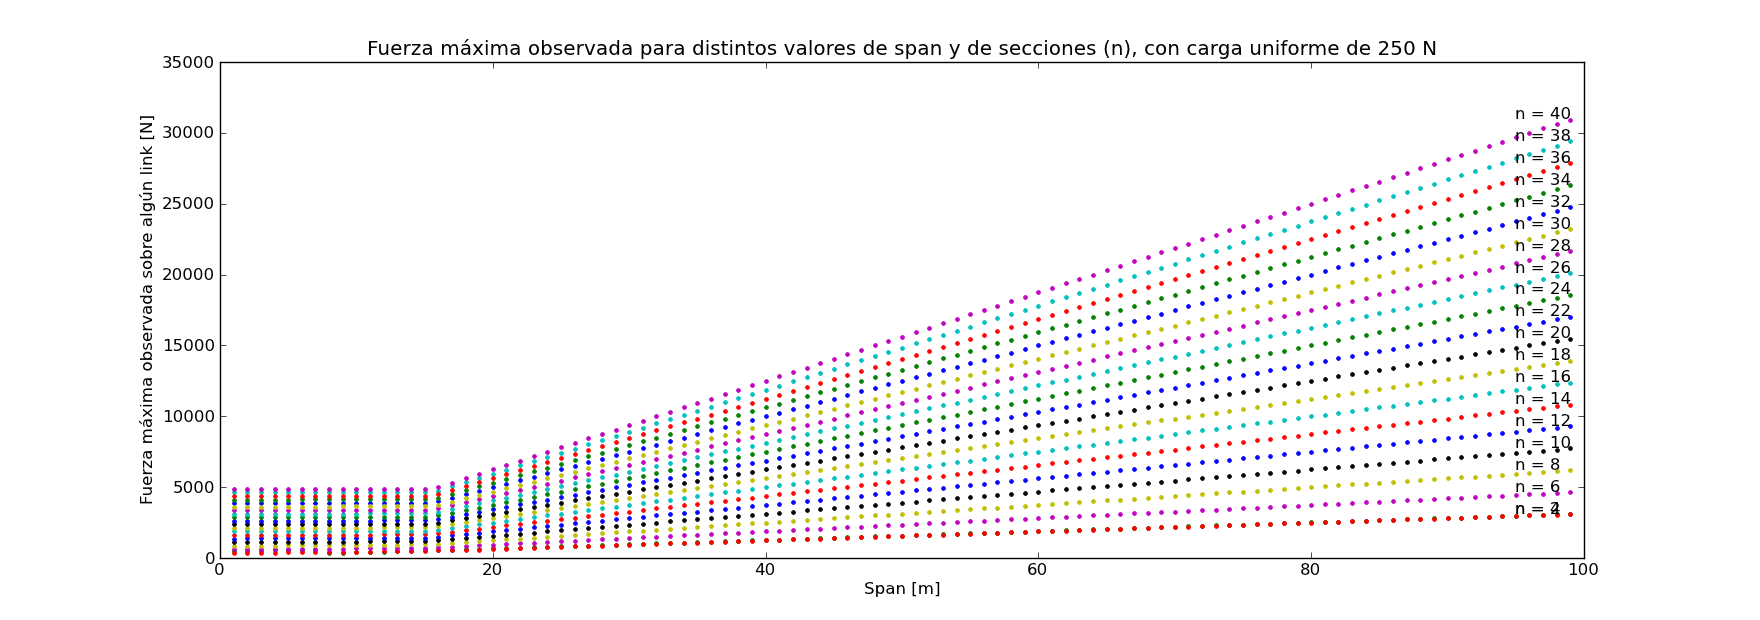
\includegraphics[width=\textwidth]{../mediciones/spanVariableDic.png}
    \caption{Fuerza máxima ejercida para distinta cantidad de secciones. Variación del valor del span.}
    \label{graf:span}
\end{figure}

Este experimento se realiz\'o con una altura igual a 4m, y una carga igual a 250N en cada junta, variando la cantidad de secciones entre 2 y 40 (siempre considerando los valores pares), y para cada uno de estos, valores de span entre 1 y 100.

Observamos en la figura \ref{graf:span} que luego de una meseta para valores bajos de span, la fuerza máxima crece linealmente tanto con el span como con el valor de $n$. Estos resultados se corresponden con la intuición: puentes más largos tienen que soportar fuerzas mayores que puentes más cortos, lo mismo que puentes con más secciones, ya que éstos tienen mayor cantidad de cargas, pues colocamos una por junta (esto tiene sentido si pensamos que pueden representar el peso de los tramos de cada sección que agregamos). También observamos que la fuerza máxima crece más rápidamente con el span para valores más grandes de $n$, lo que también podemos explicar si pensamos en que puentes con más secciones soportan mayor cantidad de carga en total.

Tambien notamos la presencia de la meseta para valores bajos de span (menores a 20m). Presentamos un detalle de esta sección en la figura \ref{graf:spanDetalle}
 
\begin{figure}[H]
  \centering
    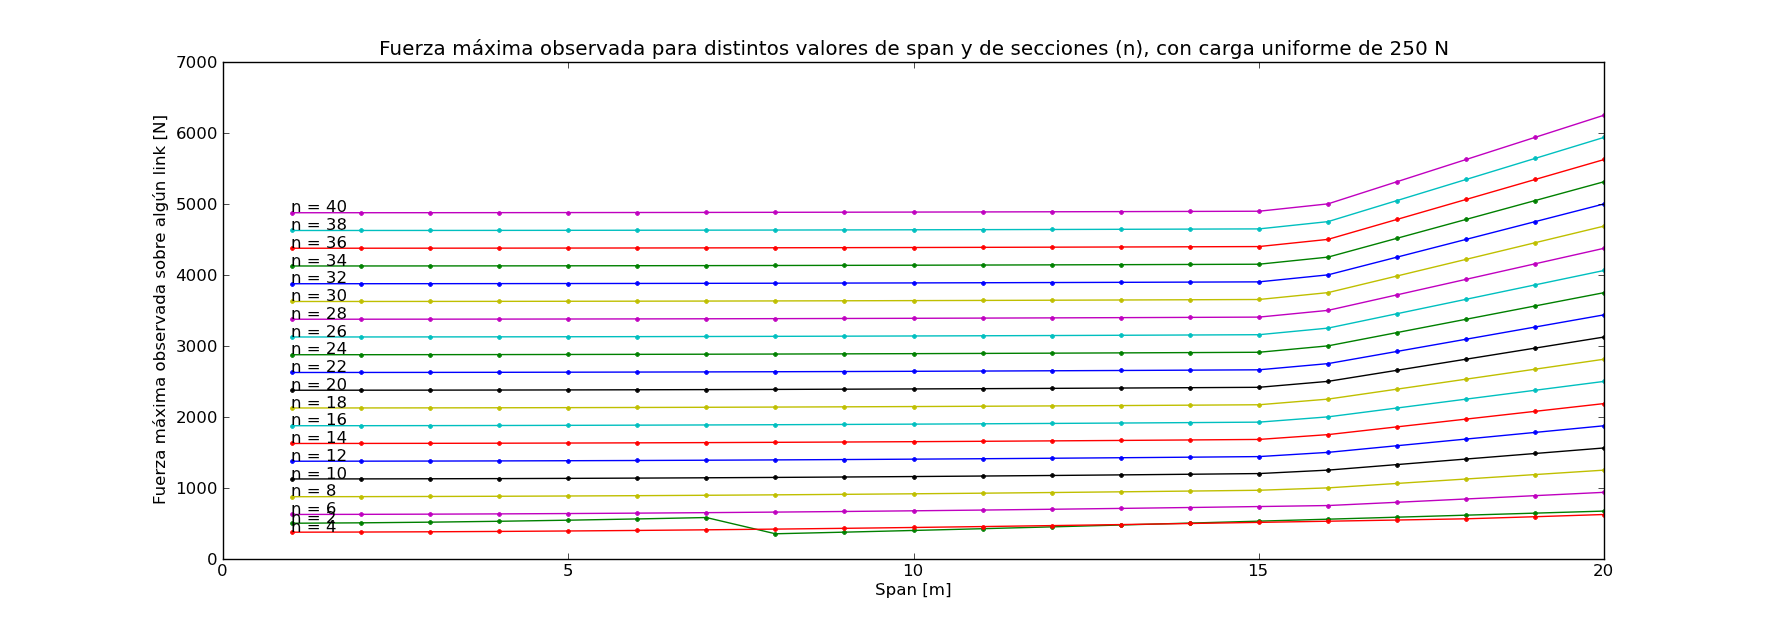
\includegraphics[width=\textwidth]{../mediciones/spanVariableDicDetalle.png}
    \caption{Detalle del gráfico de la figura \ref{graf:span}. Variación del valor del span entre 1 y 20 m.}
    \label{graf:spanDetalle}
\end{figure} 
 
Aquí observamos en la mayoría de los casos que el valor de la fuerza máxima permanece constante para las primeras mediciones, hasta valores de span de, aproximadamente, 15m. Suponemos que para estos valores estamos sobredividiendo el puente, con lo cual las cargas aplicadas no alcanzan para verdaderamente forzar la estructura. Observamos también un comportamiento particular para $n = 2$, que podemos atribuir a la forma particular que adopta el puente en este caso (por ejemplo, no tiene links oblicuos en el sentido contrario a los dos laterales). Más allá de todo esto, en todos los casos se nota con más claridad que, como dijimos antes, para los puentes con más divisiones, la fuerza máxima soportada crece más rápido. 
 
\subsubsection{Carga Variable}

\begin{figure}[H]
  \centering
    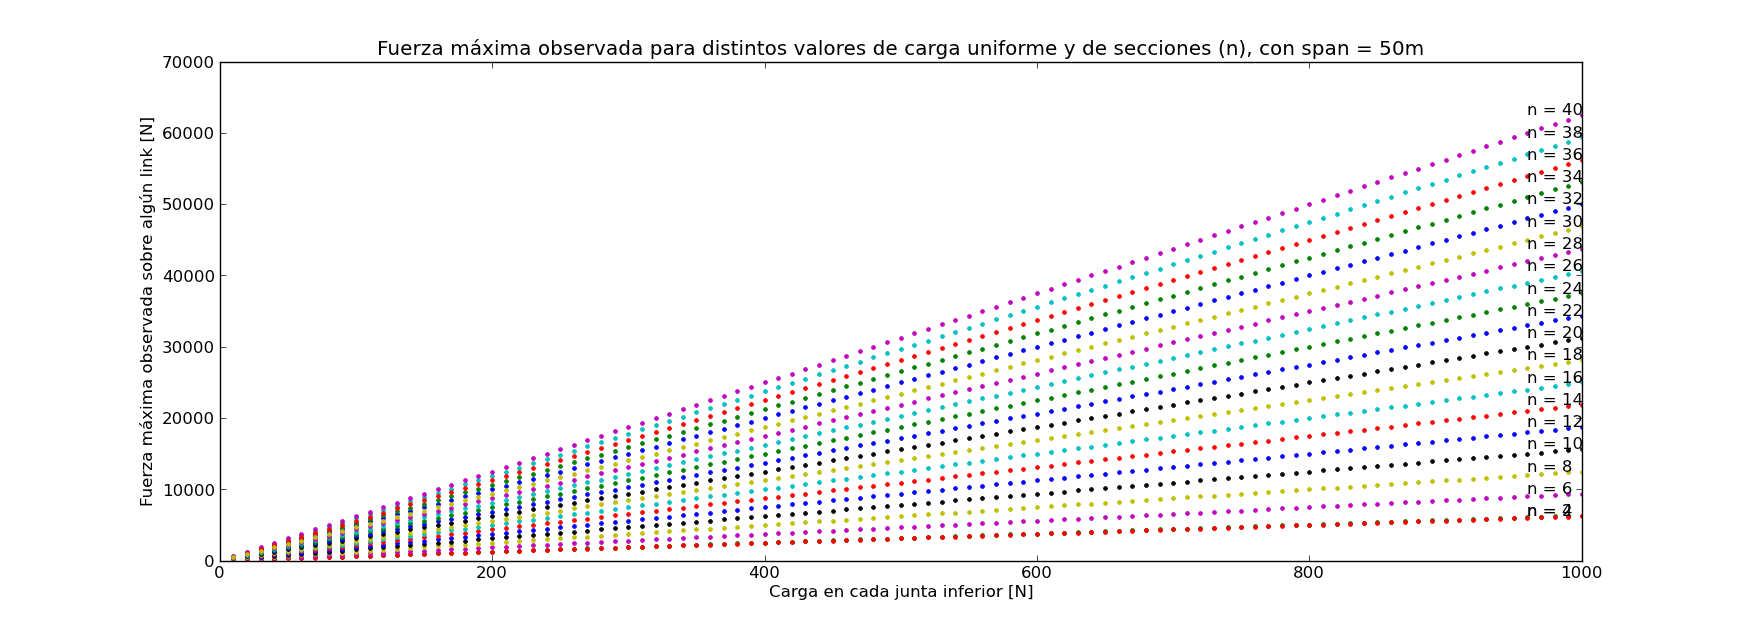
\includegraphics[width=1\textwidth]{../mediciones/cargaVariableDic.png}
    \caption{Fuerza máxima ejercida para distinta cantidad de secciones. Variación de la cantidad de carga aplicada sobre cada junta.}
   \label{graf:carga} 
\end{figure}

Este experimento se realiz\'o con una altura igual a 4m,  span igual a 50m y la carga sobre cada junta variando entre 1 y 1000N en pasos de a 10N (siendo siempre misma en todas las juntas). Tambi\'en variamos para cada una de estas situaciones la cantidad de secciones de la misma manera que en el caso anterior ($2\leq n \leq 40$, con $n$ par). Los resultados se ven en la figura \ref{graf:carga}

En este caso caben las mismas observaciones que en el caso anterior, más aún, sin la salvedad de la meseta para los valores bajos. Observamos que en estructuras más divididas (y por ende más cargadas) la fuerza soportada crece más rápido, pero siempre lo hace de manera lineal: es decir, una vez fijada la forma de la estructura del puente, la fuera máxima que se ejerce es proporcional a la cantidad de carga aplicada sobre éste.